\documentclass{article}
\usepackage{lmodern}
\usepackage[font=small,labelfont=bf]{caption}
\usepackage{mathrsfs}
\usepackage[utf8]{inputenc}
\usepackage{amsmath, fge}
\usepackage[amsmath,thmmarks]{ntheorem}
\usepackage{amssymb}
\usepackage{amsthm}
\usepackage[margin=1in]{geometry}
\usepackage{amsfonts}
\usepackage{upgreek}
\usepackage{dashbox}
\usepackage[bottom]{footmisc}
\usepackage{pdfpages}
\usepackage{graphicx}

\usepackage{mathtools}
\newlength{\temp}
\usepackage{siunitx}
\usepackage{hyperref}
\usepackage{enumitem}
\usepackage{amsbsy}
\hypersetup{
    colorlinks=true,
    linkcolor=blue,
    filecolor=magenta,      
    urlcolor=cyan,
    pdftitle={Overleaf Example},
    pdfpagemode=FullScreen,
    }
\usepackage{babel}
\usepackage{mleftright,mathtools}
\usepackage{bm}
\usepackage{fancyhdr}
\pagestyle{fancy}
\lhead{Ahou L. -  Ahou S. - Fiorini L. - Portier A.} % controls the left corner of the header
\chead{} % controls the center of the header
\rhead{Groupe 49} % controls the right corner of the header
\lfoot{} % controls the left corner of the footer
\cfoot{} % controls the center of the footer
\cfoot{~\thepage} % controls the right corner of the footer
\usepackage{titlesec}



\begin{document}


\section*{Question 1A}
\subsubsection*{Modélisation du problème}
Afin de garantir que le niveau de production ne soit pas trop bas, il nous a été demandé de maximiser le niveau minimal de production au cours de l'année. Nous allons discuter dans cette section de notre choix de modélisation pour ce problème.\\
Vous trouverez ci-dessous une table regroupant les notations utilisées dans notre modèle \footnote{Bien que $n$ et $m$ soient des constantes, nous utilisons ces notations pour alléger les formules et également pour rester dans un cadre général. Tout autre paramètre/variable sera introduit lorsque cela sera nécessaire.}:
\begin{table}[h!]
\centering
\renewcommand{\arraystretch}{1.5}% Add spacing between rows : default value is 1
\begin{tabular}{|c || c |} 
 \hline
Nom & Signification\\
 \hline\hline
 $P$  & Puissance totale à installer\\
 $\kappa \in [0, 1]$ & Proportion de la puissance totale à installer en sites \textit{offshore}\\
 $c^\text{max}_i$ & Capacité maximale installable pour le i\textsuperscript{ème} site\\
 $c_i \in [0, c_i^{\max}]$ & Capacité effectivement installée sur le i\textsuperscript{ème} site\\
 $e_i(t) \in [0,1]$ & Rendement du i\textsuperscript{ème} site au temps $t$\\
 $n$ & Nombre de sites\\
 $m$ & Nombre d'heures dans une année\\
 \hline
\end{tabular}
\caption{Table des notations utilisées pour le modèle}
\label{table:noms_des_variables}
\end{table}
\noindent \\
Parmi toutes ces variables, le problème d'optimisation porte sur le choix des $c_i$. L'idée derrière notre choix de modèle est la suivante : \\
Pour toutes les heures de l'année, nous prenons la somme de production de tous les sites en tenant compte du choix des $c_i$. Nous obtenons ainsi une fonction de la production totale en fonction du temps et dont l'allure dépend du choix des $c_i$.
Un tableau illustratif est repris ci-dessous :
\begin{table}[h!]
\centering
    \[ \begin{array}{c|cccc}
      t_i    & {t_0} & {t_1} & {\ldots}  & {t_{m-1}}\\
      \hline
      e_0(t_i) & 0.25       & 0.08   &\ldots    & 0.17 \\
      e_1(t_i) & 0.87       & 0.69   &\ldots    & 0.42 \\
      \vdots   & \vdots     & \vdots  &\vdots   & \vdots \\
      e_{n-1}(t_i) & 0.15       & 0.207   &\ldots    & 0.94 \\
      \hline
      \text{Prod. totale} &\scriptstyle \sum \limits_{i=0}^{n-1}c_i e_i(t_0) &\ldots &\ldots &\scriptstyle \sum \limits_{i=0}^{n-1}c_i e_i(t_{m-1})\\
    \end{array} \]
\caption{Table représentant les valeurs de rendement de chaque site ainsi que la production totale en fonction du temps (à titre illustratif).}
\label{table:table_rendement_illustratif}
\end{table}
\newpage
Nous cherchons donc à maximiser la valeur minimale de la production totale. Avec toutes ces informations, nous pouvons écrire notre modèle :
\begin{align*}
    \max_{c_i} \quad  
    \min_t  \biggl\{ &\sum_{i=0}^{n-1}c_i e_i(t) \biggl\} \\ 
    \sum_{i=0}^{n-1} c_i &= P\\
    \sum_{\text{\tiny offshore}}c_i &= \kappa P\\
    0 &\le \, c_i \, \le c_i^{\max} \quad \forall i \in \{0, \ldots, n-1\}
\end{align*}
Cependant, celui-ci n'est pas linéaire à cause de la fonction $\min$. Nous introduisons alors une variable intermédiaire $\gamma$ afin de remplacer le $\min$ par un problème de maximisation comme vu au cours. Le nouveau modèle, maintenant linéaire, s'écrit comme suit \footnote{La contrainte imposant que la variable $\gamma$ soit positive n'est pas nécessaire car le minimum est strictement positif et que $\gamma$ prendra cette valeur.} :
\begin{align}
    \max_{c_i, \gamma} \quad &\gamma \nonumber \\ 
    \sum_{i=0}^{n-1} c_i &= P\\
    \sum_{\text{\tiny offshore}}c_i &= \kappa P\\
    \gamma &\le \sum_{i=0}^{n-1} c_i e_i(t_j) \quad \forall j \in \{0, \ldots, m-1\}\\
    0 &\le \, c_i \, \le c_i^{\max} \quad \forall i \in \{0, \ldots, n-1\}
\end{align}
La contrainte (1) représente la puissance totale qu'il faut installer en Europe. La contrainte (2) indique qu'il faut exactement une proportion $\kappa$ de la puissance $P$ installée en \textit{offshore}. La contrainte (3) dit que la variable intermédiaire $\gamma$ ne doit pas dépasser la valeur du minimum de la fonction de production totale. Enfin, la contrainte (4) indique les bornes sur les variables $c_i$

\subsubsection*{Estimation de la taille du modèle}
\noindent
Au total, nous avons $n + 1$
variables et $m + 2$ contraintes \textbf{en plus} des "$2n$" contraintes par rapport aux bornes sur les $c_i$.\\
Cependant, lors de la résolution le \textit{solver} traduit le problème sous forme standard. Ainsi, il introduit $n + m$ variables de \textit{slack} qui correspondent au contraintes (3) et (4). Nous nous retrouvons alors avec le problème suivant : 
\begin{align*}
    \max_{c_i, \gamma, s_j, t_i} \quad  
    &\gamma \nonumber \\ 
    \sum_{i=0}^{n-1} c_i &= P\\
    \sum_{\text{\tiny offshore}}c_i &= \kappa P\\
    \gamma + s_j &= \sum_{i=0}^{n-1} c_i e_i(t_j) \quad \forall j \in \{0, \ldots, m-1\}\\
    c_i + t_i &\le c_i^{\max} \quad \forall i \in \{0, \ldots, n-1\}\\
    c_i, \gamma, s_j, t_i &\ge 0
\end{align*}
Ce qui mène à un total de $2n + m + 1$ variables et $m + n + 2$ contraintes.
\newpage
\subsection*{Question 1B}
Pour résoudre le modèle décrit dans la section précédente, nous avons utilisé la fonction \verb|linprog| de la librairie \verb|SciPy|.\\
La solution retournée par le solver pour les paramètres $P = 500000 [\mathrm{MW}]$ et $\kappa = 0.17$ nous indique qu'il y a $267$ sites sur lesquels la puissance installée est non nulle, ce qui veut dire qu'il y a $642 - 267 = 375$ sites sur lesquels il est préférable de ne pas installer d'éoliennes.\\
La répartition de puissance est représentée sur la carte ci-dessous \footnote{Les croix représentent les sites sur lesquels la puissance installée est nulle.} :

\begin{figure}[h!]
    \centering
    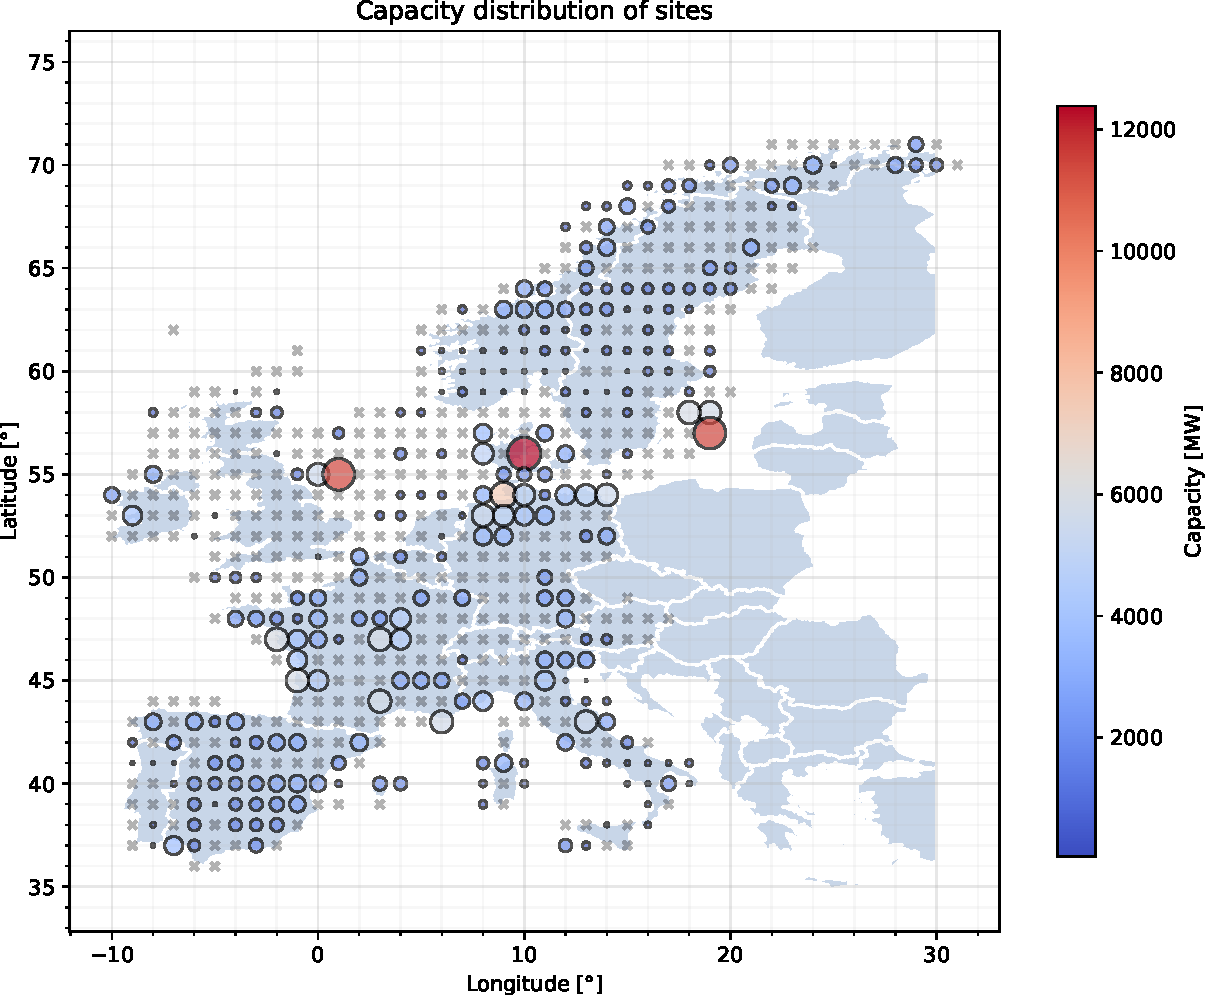
\includegraphics[scale=0.4]{Images/Partie_1/Q1/capacity_distribution.pdf}
    \caption{Carte représentant la répartition de puissance sur les différents sites d'éoliennes}
    \label{fig:capacity_distribution_partie1}
\end{figure}


Quant au temps de résolution du solver, celui-ci prend en moyenne $\approx 1.8$ secondes pour renvoyer une solution. Un graphique des performances est représenté ci-dessous :

\begin{figure}[h!]
    \centering
    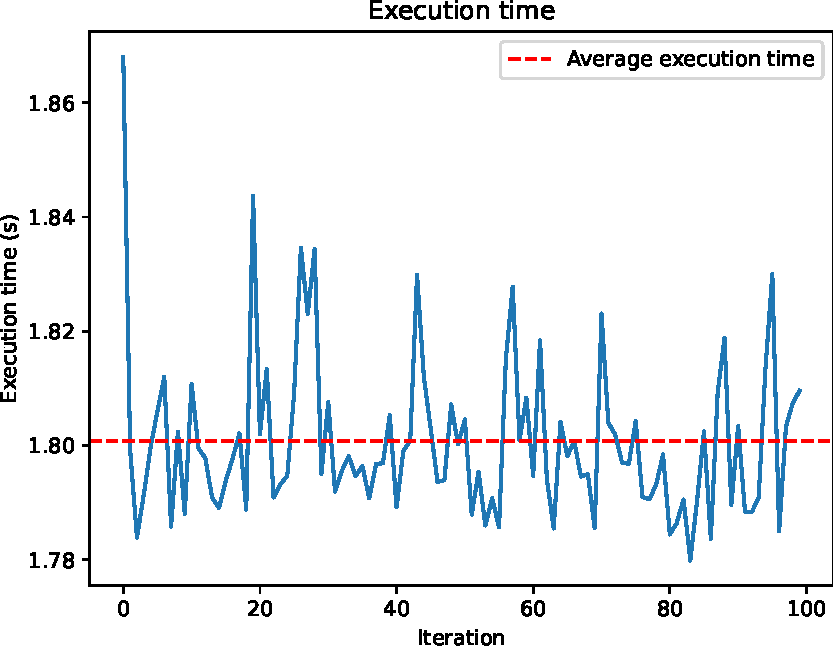
\includegraphics[scale=0.5]{Images/Partie_1/Q1/execution_time.pdf}
    \caption{Graphique du temps d'exécution sur 100 itérations}
    \label{fig:execution_time_partie1}
\end{figure}

Nous pouvons également nous intéresser à l'énergie totale produite sur l'année ainsi que sur chaque période d'une heure.
En prenant compte des rendements qui nous ont été fournis et en utilisant la solution obtenue par le solver,
il est possible de calculer, en chaque heure, l'énergie produite. Le graphique représentant la production d'énergie en fonction du temps est représenté ci-dessous :

\begin{figure}[h!]
    \centering
    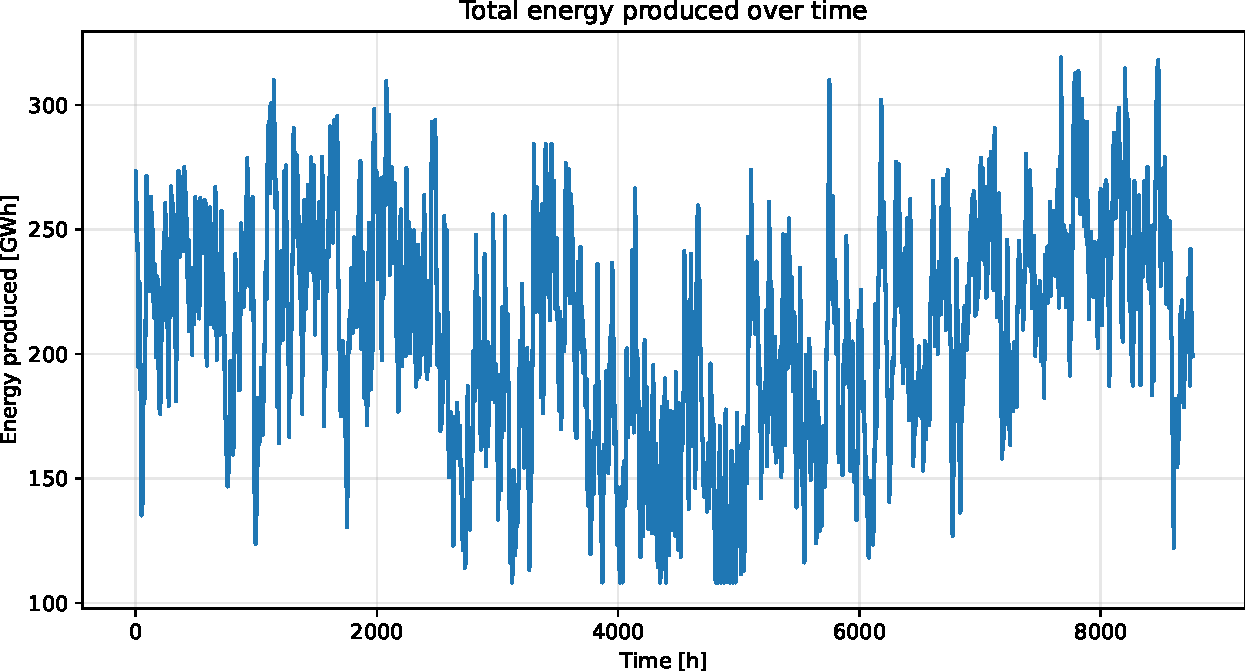
\includegraphics[scale=0.5]{Images/Partie_1/Q1/energy_produced.pdf}
    \caption{Graphique de la production d'énergie en fonction du temps}
    \label{fig:energy_produced_partie1}
\end{figure}
Et en sommant toutes les productions, nous obtenons une valeur d'environ $1828762.56 [\mathrm{GWh}]$.\\
Nous pouvons, de manière similaire, calculer le rendement de production simplement en divisant la production sur une heure par la production idéale (i.e. $P*1\mathrm{h} = P [\mathrm{MWh}]$).\\
Nous obtenons alors le graphique suivant où nous pouvons observer une moyenne de $42\%$ de rendement :

\begin{figure}[h!]
    \centering
    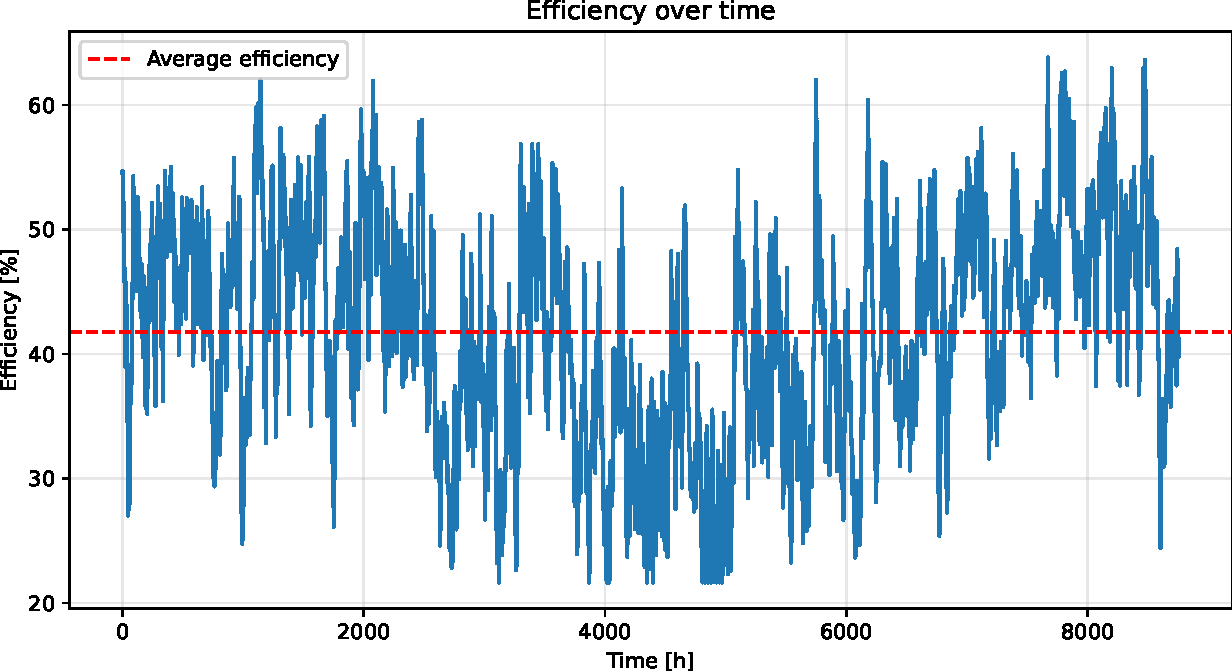
\includegraphics[scale=0.5]{Images/Partie_1/Q1/efficiency.pdf}
    \caption{graphique du rendement de production en fonction du temps}
    \label{fig:efficiency_partie1}
\end{figure}
\newpage
\section*{Question 1C}
\subsection*{(a)}
Nous avons vu au cours que les variables du problème dual associé au primal permettent de calculer la variation de la fonction objectif
lorsque l'on modifie la valeur d'une des contraintes. Lorsque l'on change la valeur de la puissance maximale installable de $P$ à $\Delta P$, la variable $y_1$ du problème dual nous indiquera de combien change
la fonction objectif (i.e. la valeur de production minimale). Nous avons donc :
\begin{equation*}
    \Delta \gamma = y_1 \Delta P
\end{equation*}

\subsection*{(b)}
Pour déterminer les sites les plus rentables sur lesquels on augmenterait la capacité dans le cas d'une modification de la puissance maximale installable, il suffit de regarder les variables duales associées aux contraintes de capacité maximale installable. En effet, ces variables nous indiquent de combien la fonction objectif varie lorsque l'on modifie la capacité maximale installable d'un site.
Nous pouvons donc résoudre le problème dual associé au primal pour obtenir ces valeurs. Après résolution, nous obtenons que les dix sites les plus intéressants sont les sites $\{241, 296, 311, 312, 313, 314, 315, 330, 434, 437\}$.\\
Cependant, lorsque nous regardons les sites où le rendement moyen est maximal, nous obtenons : $$\{ 69, 166, 167, 235, 236, 237, 434, 447, 525, 623 \}$$
Nous voyons donc que, sauf exception, il n'y pas de lien entre les sites les plus rentables quant à l'augmentation de la puissance installable et ceux où le rendement est maximal.
\newpage
\section*{Question 2A}
Dans cette deuxième question, nous avons maintenant la possibilité
d'acheter de l'énergie en chaque heure en plus de l'énergie produite par les éoliennes.
Toutefois, nous pouvons acheter qu'une quantité maximale $E_{\text{max}}$ d'énergie.\\

\subsection*{Modélisation du nouveau problème}
Pour représenter l'achat d'énergie en chaque heure de l'année, nous pouvons introduire $m$ nouvelles variables $a_j$ pour $j \in \{ 0, \ldots, m-1 \}$.\\
Notre nouveau vecteur de variables de décisions devient alors : 
\[ \bm{x} = (c_0, \ldots, c_{n-1}, a_0, \ldots, a_{m-1}, \gamma )^\intercal \]
Et notre nouveau problème devient donc :
\begin{align*}
    \max_{c_i, a_j, \gamma} \quad  &\gamma \\ 
    \sum_{i=0}^{n-1} c_i &= P\\
    \sum_{\text{\tiny offshore}}c_i &= \kappa P\\
    \gamma &\le \sum_{i=0}^{n-1} c_i e_i(t_j) + a_j \quad \forall j \in \{0, \ldots, m-1\}\\
    \sum _{j=0}^{m-1} a_j &\le E_{\text{max}}\\
    0 &\le \, c_i \, \le c_i^{\max} \quad \forall i \in \{0, \ldots, n-1\}\\
    a_j &\ge 0 \quad \forall j \in \{0, \ldots, m-1\}
\end{align*}
Où nous prenons également compte de l'énergie achetée en chaque heure dans le bilan de production d'énergie horaire (3\textsuperscript{e} contrainte).
De plus, une contrainte supplémentaire vient s'ajouter pour limiter la quantité totale d'énergie achetée. La somme des énergies achetées en chaque heure doit être inférieure à $E_{\text{max}}$ (4\textsuperscript{e} contrainte).\\
Enfin, bien que cela ne soit pas nécessaire, nous imposons que les quantités d'énergies achetées en chaque heure soient positives.

\newpage
\subsection*{Question 2B}
Nous allons maintenant résoudre ce nouveau problème pour différentes valeurs de $E_{\text{max}}$.\\
Nous avons décidé de prendre une plage de valeur allant de $0$ à $10^{9} [\mathrm{MWh}]$
\footnote{Nous avons choisi une telle plage de valeurs pour bien mettre en évidence un changement de comportement dans le graphique d'après et selon la consommation énergétique de l'UE en 2022 qui est d'environ 2.641e9[MWh] c'est une valeur tout à fait réaliste bien que la source de cette production puisse varier, source tirée du  Conseil de l'Union européenne : https://www.consilium.europa.eu/fr/infographics/how-is-eu-electricity-produced-and-sold/, consulté le 17 avril 2024 à 22h14.}
et nous résolvons le problème par incrément de $10^8 [\mathrm{MWh}]$.\\
Voici le graphique représentant le minimum de production d'énergie en fonction de la quantité d'énergie achetable :

\begin{figure}[h!]
    \centering
    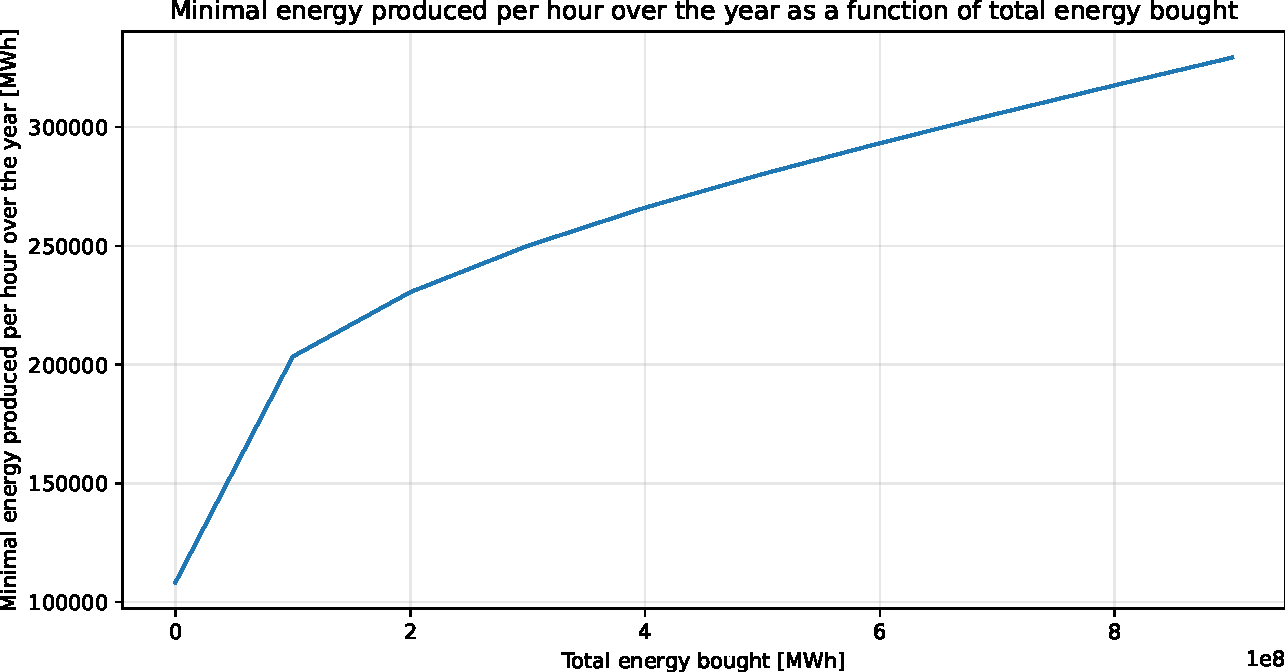
\includegraphics[scale=0.5]{Images/Partie_1/Q2/minimal_energy_produced.pdf}
    \caption{Graphique du minimum de production en fonction de l'énergie maximale achetable}
    \label{fig:minimal_energy_produced_Q2}
\end{figure}
\noindent

Le choix le plus intéressant est en fait l'endroit où la pente est maximale. En effet, en ce point là, acheter une quantité supplémentaire d'énergie amène à une augmentation maximale du minimum de production totale. Le graphique de la pente du graphique ci-dessus est représenté ci-dessous :

\begin{figure}[h!]
    \centering
    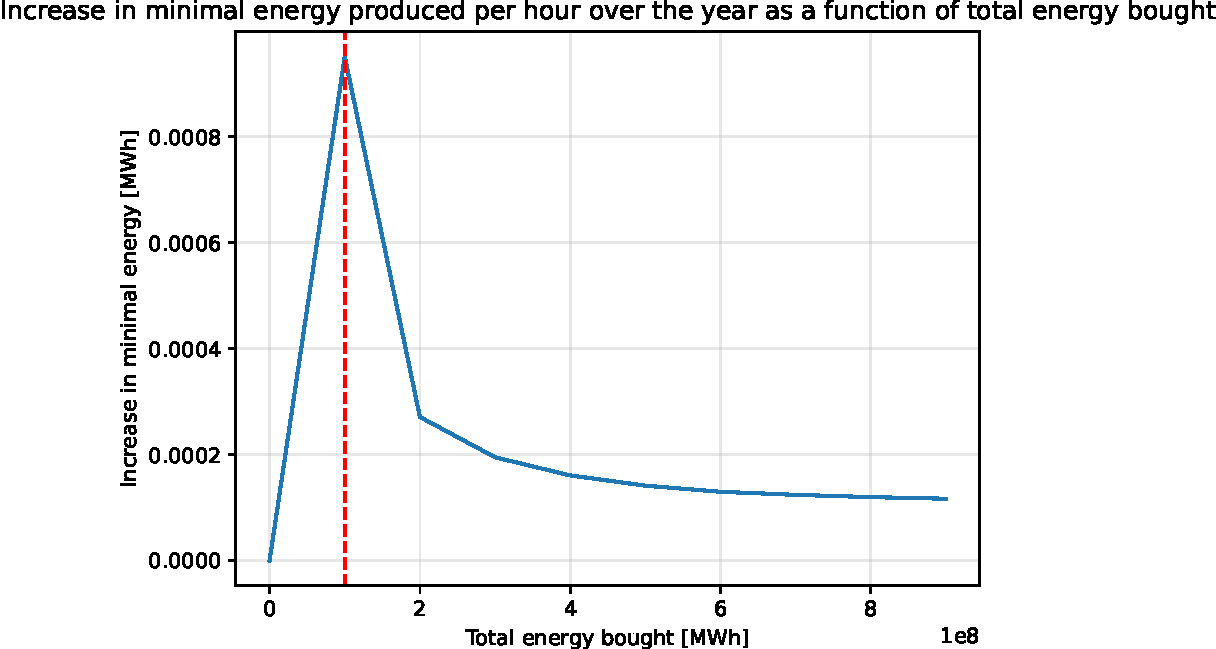
\includegraphics[scale=0.5]{Images/Partie_1/Q2/increase_minimal_energy_produced.pdf}
    \caption{Graphique de la production minimale marginale en fonction de la quantité d'énergie achetable}
    \label{fig:increase_minimal_production_Q2}
\end{figure}
Pour appuyer sur l'interprétation de ce graphique, il n'y pas un intérêt nul à acheter un autre montant d'énergie, mais à un autre niveau, chaque euro dépensé dans cet achat augmentera moins notre fonction objectif qu'à un autre seuil.

\pagebreak

Nous voyons ici que la production minimale marginale est maximale pour une valeur de $E_{\text{max}} = 1e8 [\mathrm{MWh}]$.
Nous prenons alors cette valeur pour représenter la production totale (donc en prenant compte à la fois l'énergie produite et l'énergie achetée). 

\begin{figure}[ht!]
    \centering
    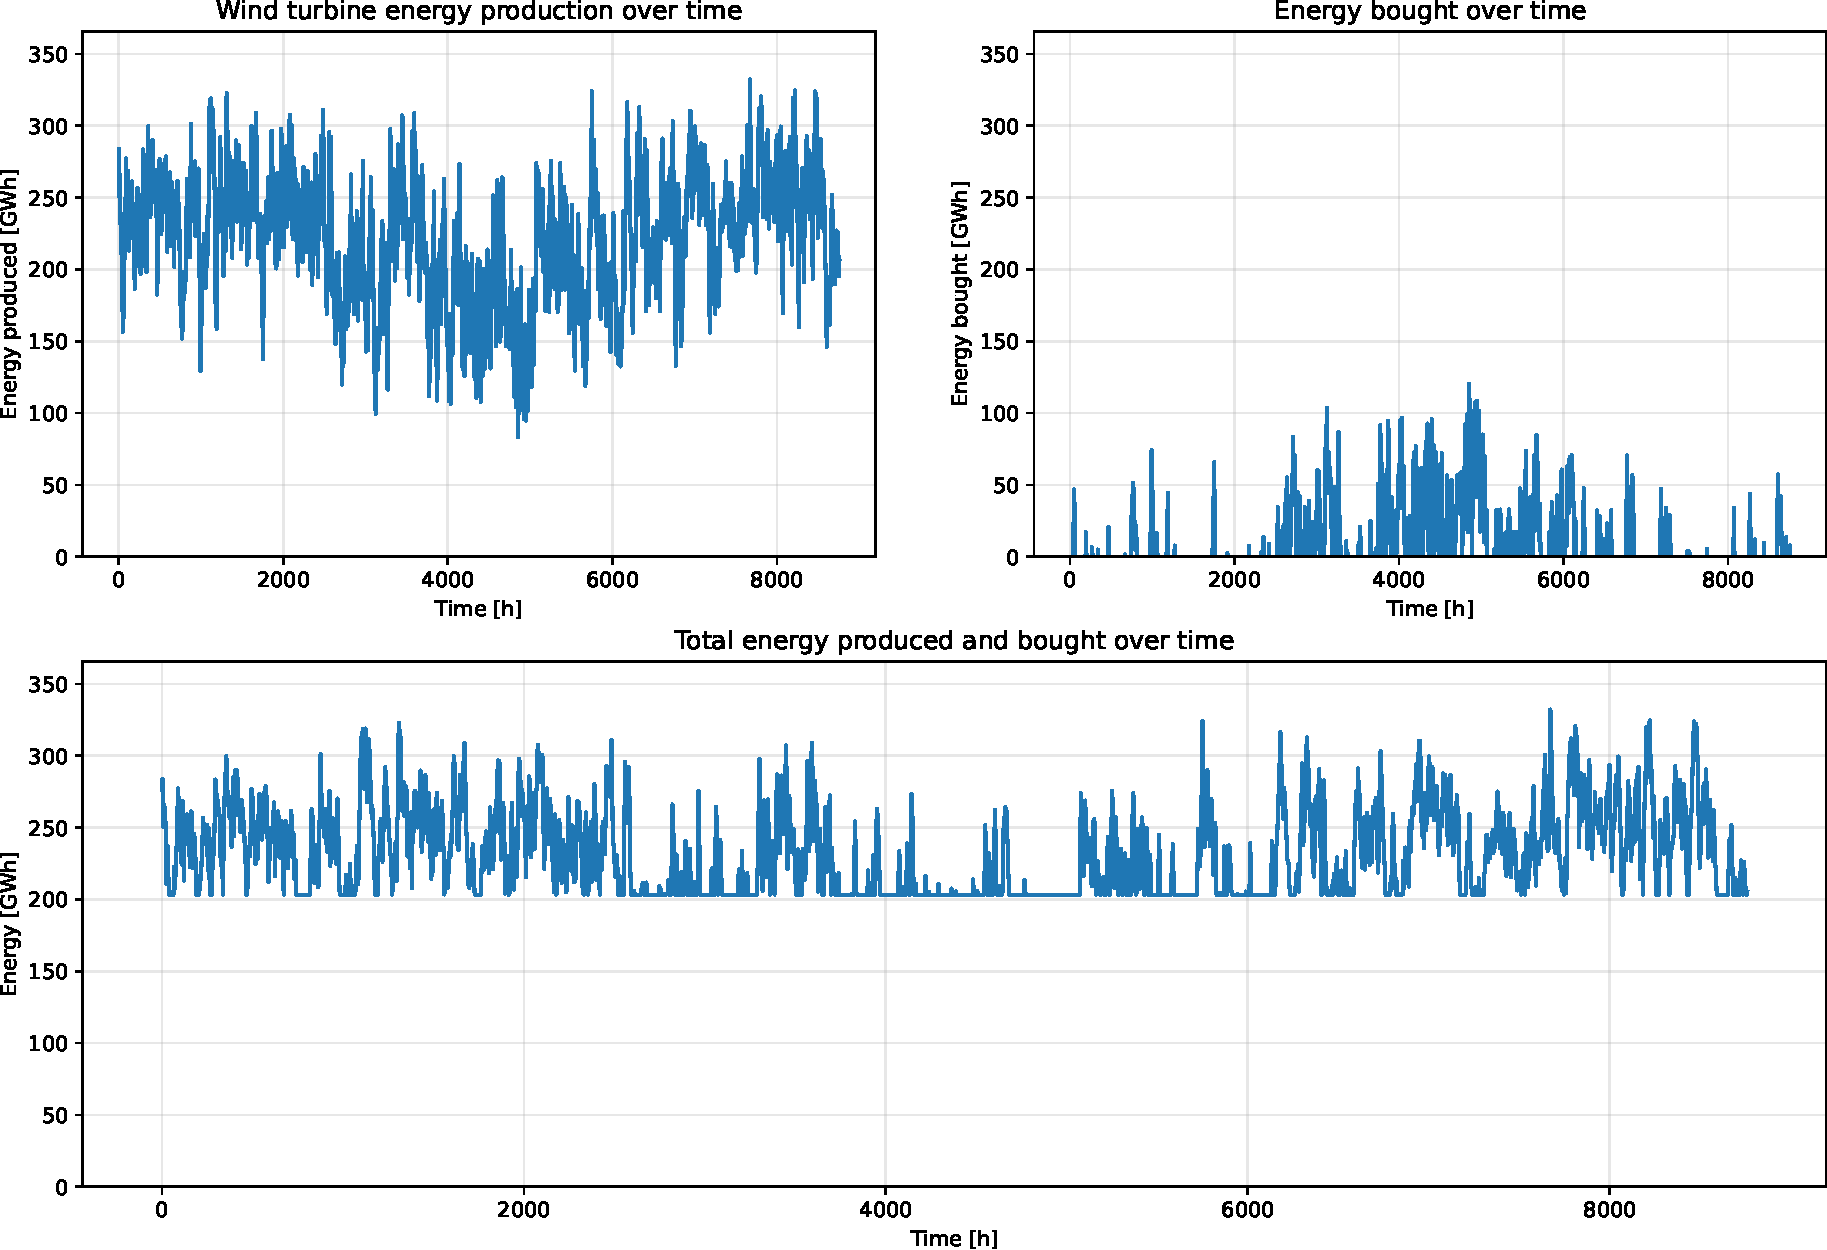
\includegraphics[scale=0.3]{Images/Partie_1/Q2/energy_produced_and_bought.pdf}
    \caption{Graphique de la production totale d'énergie pour $E_{\text{max}} = 1e8 [\mathrm{MWh}]$}
    \label{fig:total_energy_produced_and_bought_Q2}
\end{figure}
Comme nous le voyons sur la figure ci-dessus, la possibilité d'acheter de l'énergie va servir à remonter et à équilibrer les valeurs inférieures de productions d'énergie, d'où le fait que le graphique soit "plat" en-dessous.

\newpage
\section*{Question 3A}

Nous souhaitons à présent maximiser la production totale d'énergie sur l'année tout en respectant les mêmes contraintes qu'à la question 1 quant à la puissance totale et en offshore à installer.\\
Toutefois, nous souhaitons limiter la variabilité moyenne de la production d'énergie sur l'année à une valeur inférieure à $\delta P T$ où $\delta$ représente une proportion de l'énergie maximale productible sur une période de $T [h]$. Le modèle s'écrit alors :

\begin{align*}
    \max_{c_i} \quad  
    &\sum_{j = 0}^{m-1} \sum_{i = 0}^{n-1} c_i e_i(t_j) \\ 
    \sum_{i=0}^{n-1} c_i &= P\\
    \sum_{\text{\tiny offshore}}c_i &= \kappa P\\
    \left( \frac{\sum_{k = 0}^{\frac{m}{T} - 2} \Delta_k }{\frac{m}{T} - 1}\right) &\leq \delta PT\\
    0 &\le \, c_i \, \le c_i^{\max} \quad \forall i \in \{0, \ldots, n-1\}
\end{align*}

où nous avons défini pour tout $k \in \{ 0, \ldots, \frac{m}{T} - 2 \}$ :

\begin{align*}
    \epsilon_k &= \sum_{j = kT}^{(k+1)T - 1} \sum_{i = 0}^{n-1} c_i e_i(t_j) = \sum_{i=0}^{n-1} c_i \sum_{j = kT}^{(k+1)T - 1} e_i(t_j)\\
    \Delta_k &= | \epsilon_{k+1} - \epsilon_k |
\end{align*}
Et où nous supposons que m soit divisible par T, ce qui est respecté par les valeurs numériques fournies pour la résolution, si m n'était pas divisible par T, il suffirait de modifier légèrement le modèle pour qu'un intervalle soit d'une taille différente, mais cela ne changerait pratiquement rien à la formalisation.
Les valeurs absolues se trouvant dans les contraintes posent problèmes car celles-ci ne sont pas linéaires. Cependant, nous pouvons imposer deux contraintes supplémentaires pour chaque $\Delta_k$ afin de les rendre linéaires :

\begin{align*}
    \Delta_k &\leq \epsilon_{k+1} - \epsilon_k\\
    \Delta_k &\leq \epsilon_k - \epsilon_{k+1}
\end{align*}

Nous avons alors :
\begin{align*}
    \max_{c_i, \Delta_k} \quad  
    &\sum_{i=0}^{n-1} c_i \sum_{j = 0}^{m - 1} e_i(t_j) \\ 
    \sum_{i=0}^{n-1} c_i &= P\\
    \sum_{\text{\tiny offshore}}c_i &= \kappa P\\
    \left( \frac{\sum_{k = 0}^{\frac{m}{T} - 2} \Delta_k }{\frac{m}{T} - 1}\right) &\leq \delta PT\\
    \Delta_k &\ge \epsilon_{k+1} - \epsilon_k \quad \forall k \in \{ 0, \ldots, \frac{m}{T} - 2 \}\\
    \Delta_k &\ge \epsilon_k - \epsilon_{k+1}\\
    0 &\le \, c_i \, \le c_i^{\max} \quad \forall i \in \{0, \ldots, n-1\}
\end{align*}

où nous avons reformulé la fonction objectif en mettant en évidence les $c_i$.
\newpage
\section*{Question 3B}
Après résolution du modèle, nous obtenons une nouvelle répartition de la puissance installée. Cette fois-ci, nous avons 312 sites sur lesquels la puissance installée est non nulle. La répartition est représentée sur la carte ci-dessous :

\begin{figure*}[h!]
    \centering
    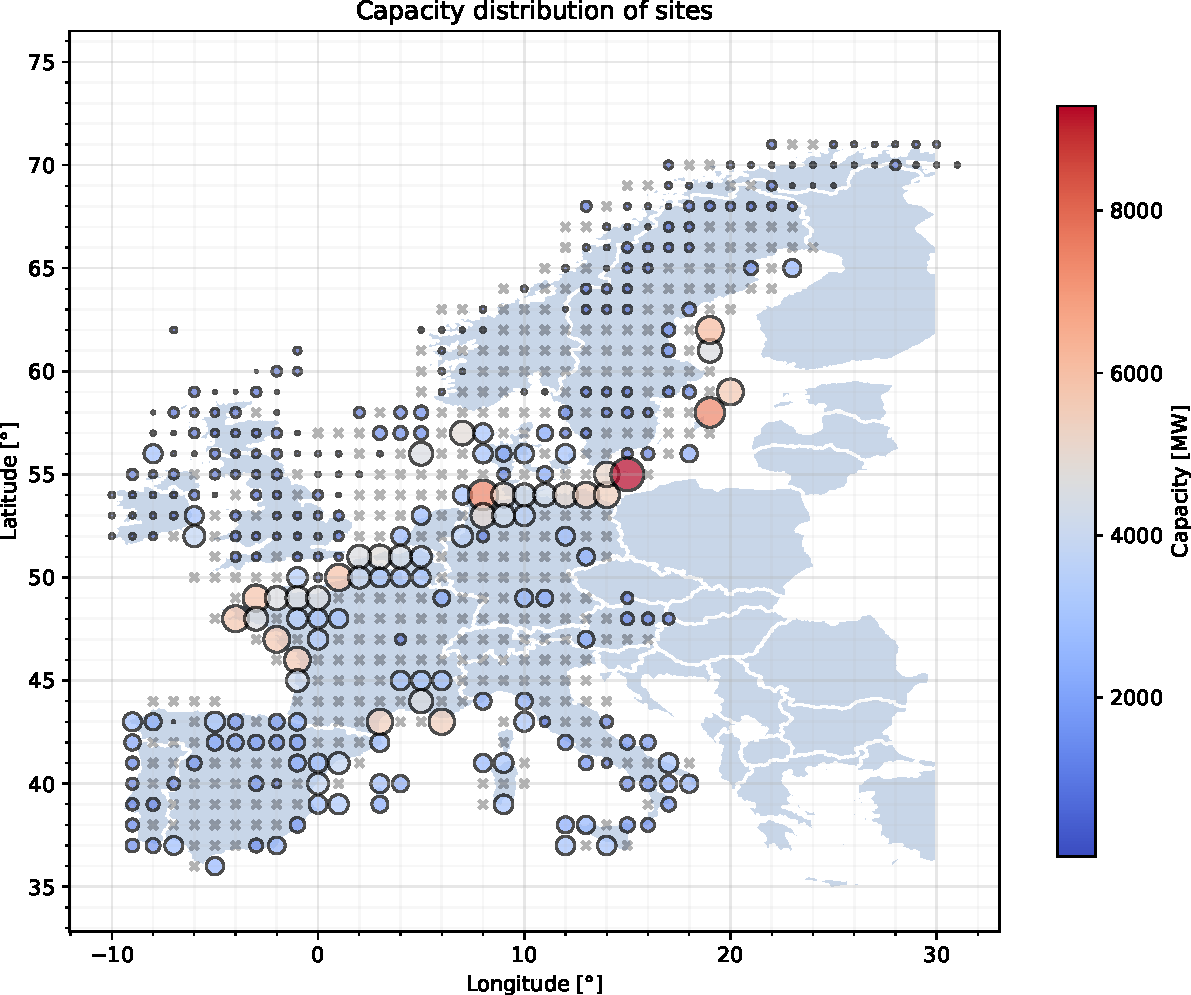
\includegraphics[scale=0.4]{Images/Partie_1/Q3/capacity_distribution.pdf}
    \caption{Carte représentant la répartition de puissance sur les différents sites d'éoliennes}
    \label{fig:capacity_distribution_partie1_Q3}
\end{figure*}

La production totale d'énergie au cours de l'année est de $1957551.15 [\mathrm{GWh}]$, contre $1828762.56 [\mathrm{GWh}]$ pour la question 1. Nous avons comparé la production en fonction du temps avec celle obtenue à la question 1 et nous avons obtenu le graphique suivant :

\begin{figure}[h!]
    \centering
    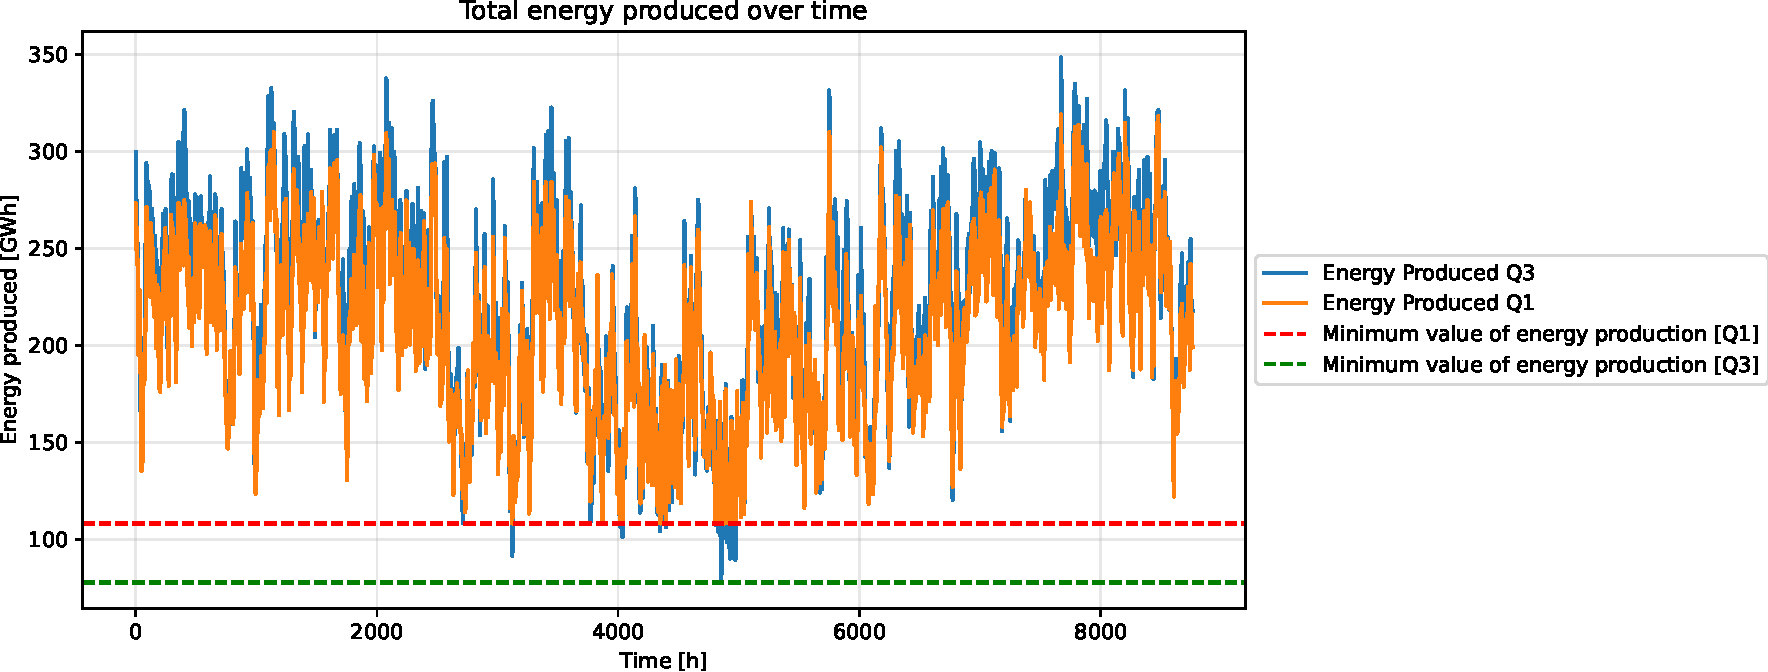
\includegraphics[scale=0.5]{Images/Partie_1/Q3/energy_produced_comparison.pdf}
    \caption{Graphique de la production d'énergie en fonction du temps}
    \label{fig:energy_produced_partie1_Q3}
\end{figure}

Comme attendu, nous observons que le minimum de production est plus élevé pour le modèle de la question 1 tandis que le modèle de la question 3 permet d'obtenir une production totale d'énergie plus élevée.\\
Lorsque nous nous intéressons à la variabilité moyenne de production, nous observons que celle-ci atteint la valeur de $\delta P T = 30 000$ (avec $\delta = 0.02, P = 500 000 [\mathrm{MW}]$ et $T = 3 [\mathrm{h}]$).\\

\begin{figure}[h!]
    \centering
    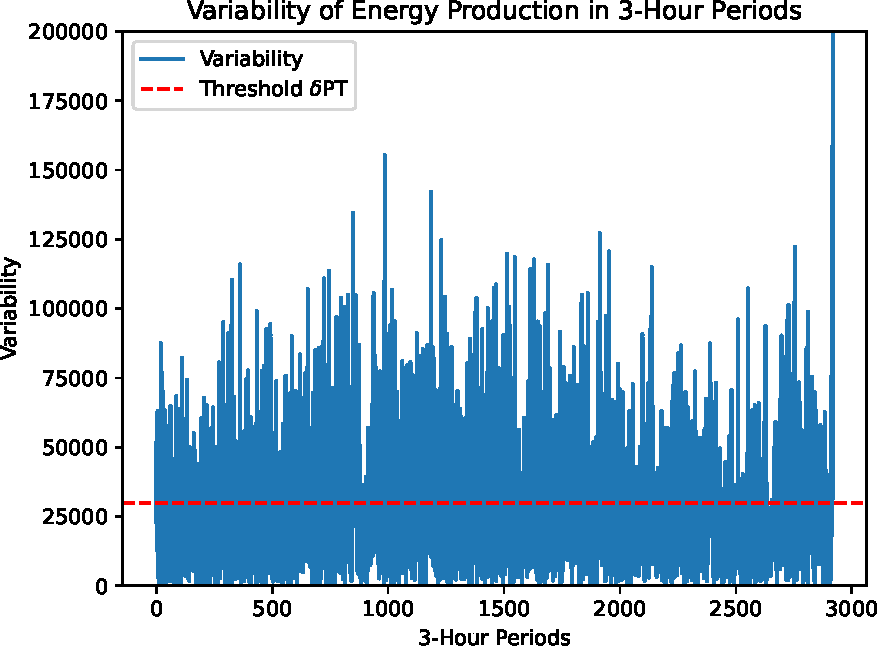
\includegraphics[scale=0.5]{Images/Partie_1/Q3/variability_comparison.pdf}
    \caption{Graphique de la variabilité de production en fonction du temps}
    \label{fig:variability_comparison_Q3}
\end{figure}
En plus du temps d'exécution moyen pour la question 1, nous avons voulu analyser l'influence du nombre de sites sur le temps de résolution de notre programme. Étant donné que c'est une opération assez lourde, nous n'avons exécuté qu'une fois le solver par changement de nombre de sites (tout en adaptant les conditions sur celui-ci afin que le problème d'optimisation reste résoluble), donc les durées enregistrées ne sont pas à priori tout à fait représentatives du temps nécessaire en général, mais arrivent empiriquement à dresser une bonne allure de ce à quoi nous devrions nous attendre.

\begin{figure}[h!]
    \centering
    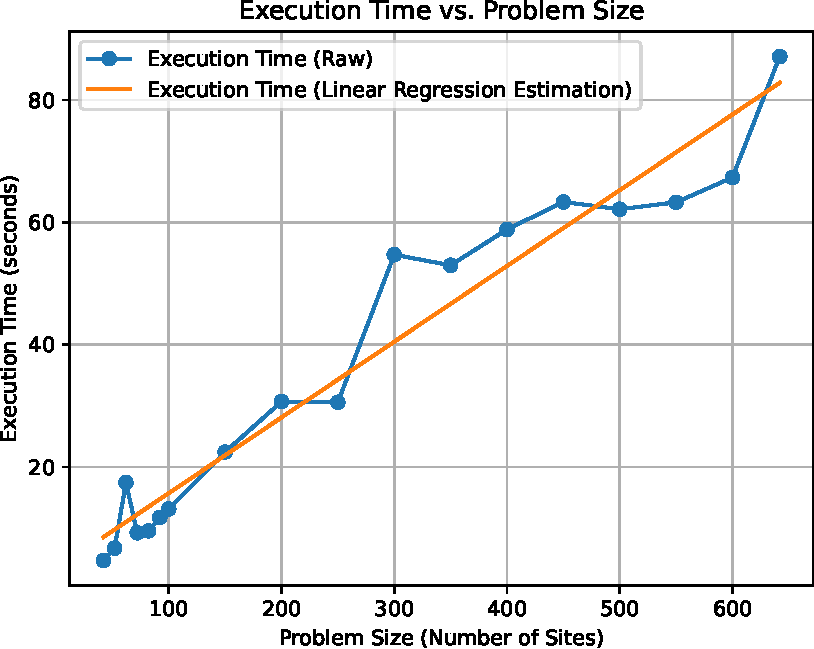
\includegraphics[scale=0.5]{Images/Partie_1/Q3/execution_time_vs_problem_size.pdf}
    \caption{Graphique du temps d'exécution de \textit{linprog} en fonction du nombre de sites}
    \label{fig:execution_time_vs_problem_size_Q3}
\end{figure}
Le résultat que nous observons semble assez cohérent, le solver semble ne pas subir une croissance plus que linéaire en fonction du nombre de sites (cela aurait été sûrement un cas similaire si nous avions fait varier le nombre d'heures (8760) au lieu des sites). Pourtant, rajouter énormément de variables pour une résolution à la main aurait probablement complexifié la chose plus que linéairement, chose qui montre que \textit{linprog} se comporte assez bien, intuitivement. Cela reste cependant assez peu d'informations pour juger de la qualité du solver, mais en tout cas, pour ce problème, et ce nombre de variables, il ne semble pas prendre un temps exponentiel de résolution, ce qui nous est utile.

\subsection*{Conclusion}
Voici un tableau récapitulatif reprenant les caractéristiques de chacun des trois modèles présentés dans cette première partie du projet :
\begin{center}
    \begin{tabular}{c| c c c }
        Caractéristiques & Question 1 & Question 2 & Question 3\\
        \hline
        Nombre de sites avec productions non nulles & 267 & 267 & 312\\
        Production totale d'énergie $[\mathrm{GWh}]$& $1828762.56$ & $2035764.02$ & $1957551.15$\\
        Minimum de production $[\mathrm{MWh}]$ & $108249.48$ & $203397.45$ & $77793.64$\\
        Maximum de production $[\mathrm{MWh}]$ & $319059.43$ & $332235.91$ & $348449.77$\\
        Variabilité moyenne de production & $28742.42$ & $20511.61$ & $29789.53$\\
        \hline
    \end{tabular}
\end{center}

\medskip
Bien que le modèle de la question 3 avait pour but de limiter la variabilité moyenne de production, nous observons que celle-ci est plus élevée que pour les modèles des question 1 et 2. Cela est dû au fait que le modèle de la question 3 cherche à maximiser la production totale d'énergie, ce qui peut amener à des différences élevées entre les maximums et minimums de productions.\\
Nous voyons cependant bien les différences de comportement entre les trois modèles quant aux minima et maxima de production d'énergie. Le modèle de la question 2 permet d'obtenir un minimum de production plus élevé que les deux autres modèles  car l'objectif est de maximiser ce minimum avec la possibilité d'acheter de l'énergie. Le modèle de la question 3 permet d'obtenir une production totale d'énergie plus élevée que le modèle de la question 1 et 2 (sans compter la possibilité d'achat) car l'objectif est de maximiser cette production totale.\\

\newpage
\thispagestyle{empty}
\section*{Contributions au projet du groupe 49}
\begin{table}[h]
    \centering
    \begin{tabular}{|c|c|p{6cm}|}
        \hline
        \textbf{Nom} & \textbf{Noma} & \textbf{Contribution} \\
        \hline
        AHOU Lucas & 3594-22-00 & Réponse aux questions et rédaction principale du fichier \LaTeX \\
        \hline
        AHOU Samuel & 4408-19-00 & Utilisation des paquets afin de générer les graphiques contenant les cartes et réponses aux questions \\
        \hline
        FIORINI Lucien & 7502-22-00 & Formalisation mathématique et relecture du code \\
        \hline
        PORTIER Adrien & 5337-22-00 & Écriture du code du notebook et formalisation mathématique \\
        \hline
    \end{tabular}
\end{table}

\end{document} 